% Options for packages loaded elsewhere
\PassOptionsToPackage{unicode}{hyperref}
\PassOptionsToPackage{hyphens}{url}
\PassOptionsToPackage{dvipsnames,svgnames,x11names}{xcolor}
%
\documentclass[
  12pt,
]{article}
\usepackage{amsmath,amssymb}
\usepackage{lmodern}
\usepackage{iftex}
\ifPDFTeX
  \usepackage[T1]{fontenc}
  \usepackage[utf8]{inputenc}
  \usepackage{textcomp} % provide euro and other symbols
\else % if luatex or xetex
  \usepackage{unicode-math}
  \defaultfontfeatures{Scale=MatchLowercase}
  \defaultfontfeatures[\rmfamily]{Ligatures=TeX,Scale=1}
\fi
% Use upquote if available, for straight quotes in verbatim environments
\IfFileExists{upquote.sty}{\usepackage{upquote}}{}
\IfFileExists{microtype.sty}{% use microtype if available
  \usepackage[]{microtype}
  \UseMicrotypeSet[protrusion]{basicmath} % disable protrusion for tt fonts
}{}
\makeatletter
\@ifundefined{KOMAClassName}{% if non-KOMA class
  \IfFileExists{parskip.sty}{%
    \usepackage{parskip}
  }{% else
    \setlength{\parindent}{0pt}
    \setlength{\parskip}{6pt plus 2pt minus 1pt}}
}{% if KOMA class
  \KOMAoptions{parskip=half}}
\makeatother
\usepackage{xcolor}
\usepackage[margin=1in]{geometry}
\usepackage{longtable,booktabs,array}
\usepackage{calc} % for calculating minipage widths
% Correct order of tables after \paragraph or \subparagraph
\usepackage{etoolbox}
\makeatletter
\patchcmd\longtable{\par}{\if@noskipsec\mbox{}\fi\par}{}{}
\makeatother
% Allow footnotes in longtable head/foot
\IfFileExists{footnotehyper.sty}{\usepackage{footnotehyper}}{\usepackage{footnote}}
\makesavenoteenv{longtable}
\usepackage{graphicx}
\makeatletter
\def\maxwidth{\ifdim\Gin@nat@width>\linewidth\linewidth\else\Gin@nat@width\fi}
\def\maxheight{\ifdim\Gin@nat@height>\textheight\textheight\else\Gin@nat@height\fi}
\makeatother
% Scale images if necessary, so that they will not overflow the page
% margins by default, and it is still possible to overwrite the defaults
% using explicit options in \includegraphics[width, height, ...]{}
\setkeys{Gin}{width=\maxwidth,height=\maxheight,keepaspectratio}
% Set default figure placement to htbp
\makeatletter
\def\fps@figure{htbp}
\makeatother
\setlength{\emergencystretch}{3em} % prevent overfull lines
\providecommand{\tightlist}{%
  \setlength{\itemsep}{0pt}\setlength{\parskip}{0pt}}
\setcounter{secnumdepth}{5}
\newlength{\cslhangindent}
\setlength{\cslhangindent}{1.5em}
\newlength{\csllabelwidth}
\setlength{\csllabelwidth}{3em}
\newlength{\cslentryspacingunit} % times entry-spacing
\setlength{\cslentryspacingunit}{\parskip}
\newenvironment{CSLReferences}[2] % #1 hanging-ident, #2 entry spacing
 {% don't indent paragraphs
  \setlength{\parindent}{0pt}
  % turn on hanging indent if param 1 is 1
  \ifodd #1
  \let\oldpar\par
  \def\par{\hangindent=\cslhangindent\oldpar}
  \fi
  % set entry spacing
  \setlength{\parskip}{#2\cslentryspacingunit}
 }%
 {}
\usepackage{calc}
\newcommand{\CSLBlock}[1]{#1\hfill\break}
\newcommand{\CSLLeftMargin}[1]{\parbox[t]{\csllabelwidth}{#1}}
\newcommand{\CSLRightInline}[1]{\parbox[t]{\linewidth - \csllabelwidth}{#1}\break}
\newcommand{\CSLIndent}[1]{\hspace{\cslhangindent}#1}
\usepackage{polyglossia}
\setmainlanguage{english}
\usepackage{booktabs}
\usepackage{caption}
\captionsetup[table]{skip=10pt}
\xpglanginauxtrue
\ifLuaTeX
  \usepackage{selnolig}  % disable illegal ligatures
\fi
\IfFileExists{bookmark.sty}{\usepackage{bookmark}}{\usepackage{hyperref}}
\IfFileExists{xurl.sty}{\usepackage{xurl}}{} % add URL line breaks if available
\urlstyle{same} % disable monospaced font for URLs
\hypersetup{
  pdftitle={Nuclear Explosion Tests},
  pdfauthor={Soyugur, Cankat},
  colorlinks=true,
  linkcolor={Maroon},
  filecolor={Maroon},
  citecolor={Blue},
  urlcolor={blue},
  pdfcreator={LaTeX via pandoc}}

\title{Nuclear Explosion Tests}
\author{Soyugur, Cankat\footnote{20080501, \href{https://github.com/cnktxd/Final.git}{Github Repo}}}
\date{}

\begin{document}
\maketitle
\begin{abstract}
This research is about the nuclear explosion tests that happened between 1945 and 1998. The norm of nuclear warfare and nuclear testing is important in politics as these tests were used as a show of power. In this research the tests of the USA and France will be discussed with regards to the question ``Were the USA's nuclear tests more effective than the French nuclear tests on average?''. This effectiveness will be compared with the upper yields of these tests. The main method used in this research is a Two-Sided T-Test, the reason why I used this method is in order to conclude an understandable comparison for the 2 countries, the T-Test was the most efficient way of doing so. I found that the USA's nuclear tests were more effective even by looking at the graphs. The T-Test also gave a hint at this conclusion as the differance was somewhat significant in a statistical way.
\end{abstract}

\hypertarget{introduction}{%
\section{Introduction}\label{introduction}}

The purpose of my work is to investigate the dataset about nuclear explosions. By editing the given dataset, I removed the rows that included ``NA'' values and also deleted the columns that were no use to me such as ``magnitude\_body'' and ``magnitude\_surface''. The other variables are: date\_long(Shows the complete date of the testing), year, country(Which country conducted the test), region(Where the test was conducted at), latitude, longitude, depth, yield\_lower, yield\_higher, purpose(Why the test was conducted for), name(Name of the detonated warhead) and type(How the nuclear test was conducted).

The question I decided on is ``Were the USA's nuclear tests more effective than the French nuclear tests on average?''. The question is related with the 4 articles I have found and they provided me with extra information I stated in the literature review section. Also from the dataset, I can gather the needed data by using some functional codes.

For the analysis, I will compare the occurances of US nuclear tests and the French nuclear tests with regards to the upper and lower yield to understand the effectiveness of the tests. I will be using a T-Test for this research in order do a better comparison.

The test is two-sided. The null hypothesis is ``USA's nuclear tests were more efficent than the French ones. The alternative hypothesis is''USA's nuclear tests weren't more efficent than the French ones.''

\hypertarget{literature-review}{%
\subsection{Literature Review}\label{literature-review}}

Even though the literature I found is mostly made of data from the tests of nuclear weapons, the 4 articles and reports I found also include and give valuable information about the question.

The US is shown to have conducted almost all of it's nuclear tests in Nevada Test Site or NTS as an abbreviation. Before the tests at NTS, USA conducted it's tests at various places around the pacific as given in quote: (\protect\hyperlink{ref-bergkvist:2000}{Nils-Olov Bergkvist, 2000}) ``Nuclear weapon development continued in the USA and tests were conducted in 1946-62 at various atolls and islands in the Pacific Ocean. The first hydrogen bomb was tested in 1951, at Enewetak Atoll, then part of a UN Trust territory administered by the USA, now part of the Marshall Islands.''.In the introduction section of the article from (\protect\hyperlink{ref-anauxefs:2016}{Seantel Anaïs, 2016}) it is stated how many tests were conducted and how big of a yield the tests had at the NTS is stated, which is also relevant to my first question with quote: ``At the Nevada Test Site (NTS) northwest of Las Vegas, Nevada, 928 above- and below-ground nuclear tests occurred between 1951 and 1992. There were nearly 90 tests at the NTS in 1962 alone (NTS interviewee). Bombs of 61 and 74 kilotonnes were detonated at the NTS during the 1950s -- by contrast, the bomb dropped on Hiroshima had a nuclear yield of approximately 15 kilotonnes.''

Information about the French nuclear tests are less shared to the public than the USA's nuclear tests because of various reasons. These reasons include the failures of the tests, the health problems created by the test as stated in (\protect\hyperlink{ref-danielsson:1984}{Danielsson, 1984}) with quote: ``Most political, church and civic leaders in French Polynesia immediately voiced strong fears that any nuclear tests made in the Tuamotus might, as the American tests did in Micronesia, adversely affect the health of the 7 000 people living there.'' and ``By the beginning of July 1966, after three years of intense preparations, the Moruroa testing base was operational. The first bomb was placed on a barge anchored in the lagoon and detonated. The result was a catastrophe-all the water contained in the shallow reef basin was sucked up into the air and then rained down, covering all islets with heaps of irradiated fish and clams, whose slowly rotting flesh continued to stink for weeks.'' However, from (\protect\hyperlink{ref-willis:2006}{Willis, 2006}) it can be said that the testing of the French warheads were mostly conducted in the French Polynesia, especially in Moruroa and Tuamotus islands, but these were also not that effective and therefore, were not reported as after the failure of the first few tests, the types of which were ``SURFACE'' and ``TOWER'', the French converted to different types of testing types.

\hypertarget{data}{%
\section{Data}\label{data}}

I found this data from ``\url{https://github.com/rfordatascience/tidytuesday}''. The dataset was hard to find as I wanted to conduct a research on some topic that I was interested in. The main source of the dataset is SIPRI, Stockholm International Peace Research Institute, that conducts researches about anything from wars to illegal weapons trade.

The main dataset is named ``nuclear\_explosions1''. With cropping the rows that had ``NA'' values, I had 1382 entries in total. This was the only edit I did on the main dataset. Other than this, I had to create a subset named ``comparison1'' in order to conduct a test relevant to my question. This subset has 2 columns: ``country'' and ``upper\_yield''. Since my question is about the effectiveness of the tests between the US and France, I deleted the rows that had the names other than USA and France. By doing this, I had 1236 entries in total inside ``comparison1''.

The summary statistics shows the upper yield of the 2 countries seperately. Table 1 shows the statistics of France and table 2 shows the statistics of the US. Each table shows the mean, standard deviation(Given as ``Std.Dev''), minimum value of the tests(Given as ``Min''), median value of the tests(Given as ``Median'') and finally, the maximum value of the tests(Given as ``Max'').

\begin{verbatim}
## \begin{table}[ht]
## \centering
## \caption{France Nuclear Test Statistics} 
## \label{tab:summary}
## \begin{tabular}{lccccc}
##   \toprule
##  & Mean & Std.Dev & Min & Median & Max \\ 
##   \midrule
## yield\_upper & 103.89 & 213.23 & 0.00 & 20.00 & 1000.00 \\ 
##    \bottomrule
## \end{tabular}
## \end{table}
\end{verbatim}

\begin{verbatim}
## \begin{table}[ht]
## \centering
## \caption{USA Nuclear Test Statistics} 
## \label{tab:summary}
## \begin{tabular}{lccccc}
##   \toprule
##  & Mean & Std.Dev & Min & Median & Max \\ 
##   \midrule
## yield\_upper & 226.34 & 1094.94 & 0.00 & 20.00 & 15000.00 \\ 
##    \bottomrule
## \end{tabular}
## \end{table}
\end{verbatim}

\hypertarget{methods-and-data-analysis}{%
\section{Methods and Data Analysis}\label{methods-and-data-analysis}}

I need to conduct a T-Test since my question is related to the average results of two different country's nuclear tests so I need to conduct a Two-Sided T-Test. Before conducting this test, I need to find out whether or not the variances are equal. This is needed because if the variances are equal, I can conduct a standard Two-Sided T-Test and if they are not, I have to conduct a Welch Two-Sided T-Test.

In order to find out if the variances between the two variables are equal or not, I have to conduct an Ansari-Bradley Test.

My Hypothesis For Ansari-Bradley Test:

H0: Variances are equal to 1.

H1: Variances are not equal to 1.

\begin{verbatim}
## 
##  Ansari-Bradley test
## 
## data:  yield_upper by country
## AB = 62861, p-value = 0.7139
## alternative hypothesis: true ratio of scales is not equal to 1
\end{verbatim}

The standard confidence interval of the Ansari-Bradley Test is 95 percent and the p value that came out from the test is 0.7139. With this, I failed to reject the null hypothesis that the variances are equal to 1 since the p-value is within the are of acceptance.

From these results, I can safely conduct a Two-Sided T-Test rather than a Welch T-Test.

My Hypothesis For the Two-Sided T-Test:

H1: The nuclear tests of the US were more effective than the nuclear tests of France.

H0: The nuclear tests of the US were not more effective than the nuclear tests of France.

\begin{verbatim}
## 
##  Two Sample t-test
## 
## data:  yield_upper by country
## t = -1.6024, df = 1234, p-value = 0.1093
## alternative hypothesis: true difference in means between group FRANCE and group USA is not equal to 0
## 95 percent confidence interval:
##  -272.37008   27.47237
## sample estimates:
## mean in group FRANCE    mean in group USA 
##             103.8889             226.3377
\end{verbatim}

This T Test allows me to analyse the effectiveness of the nuclear tests of the US and France. It can be said that the populations are not normally distributed. From the T-Test, it can be seen that France has a mean of 103.8889 while the tests of the US has a mean of 226.3377.

The T-Test gives an outcome that the nuclear tests of the US were way more effective than the ones of France. The first reason for this is that the p value(Which is 0.1093),is within the area of acceptance, since the confidence interval is 95 percent. With this, the null hypothesis can be accepted, meaning that I failed to reject the hypothesis.

The second and the final reason is the difference between the means of two countries in the T-Test is significant and gives the conclusion that the tests of the US were more effective since the difference between the two means of the US and France are quite large and the difference is in the favor of the US.

Looking at the graphs below gives a clearer sign that the US's tests were more effective.

\newpage

First graph \ref{fig:plot1} shows the nuclear test ratios of the US and France that has an upper yield (Abbrevatiated for a thousand as hundreds.) lower than 200. It can be seen that the difference of these tests are not significant as they look close. With this, it can't be said that the tests of these countries with the filtered yield is more significant than one another. However, the graph below gives the result needed.

\begin{figure}

{\centering 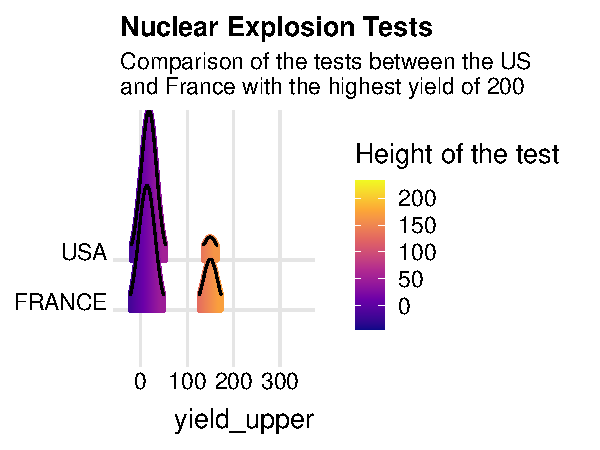
\includegraphics{project_files/figure-latex/plot1-1} 

}

\caption{Nuclear Explosion Tests}\label{fig:plot1}
\end{figure}

\newpage
\begin{figure}

{\centering 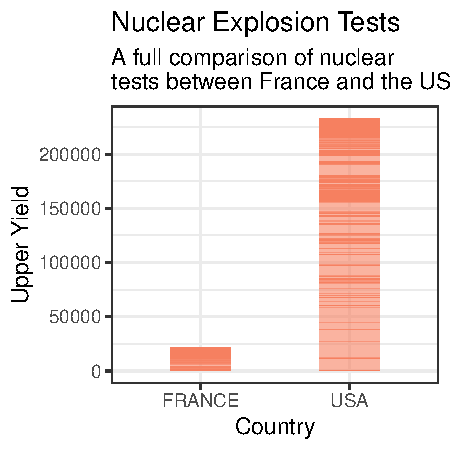
\includegraphics{project_files/figure-latex/plot2-1} 

}

\caption{Complete Comparison}\label{fig:plot2}
\end{figure}

\ref{fig:plot2} shows the bar plotted tests of both countries. The x axis has the names of both countries and the y axis shows the upper yield of the nuclear tests of those countries. It can be clearly seen that the US's nuclear tests goes all the way up to the point above 200000. Meanwhile French tests only reach a point that is below 50000 and around 10000 upper yield. This is also a clear indication that the tests of the US were way more effective than the ones of France's.

Another point that we can understand from this graph is that the US conducted way more nuclear tests in all compared to France. From the dataset ``comparison1'', it can be seen that France only conducted 190 nuclear tests in total whereas the US conducted 1046 nuclear tests. From this, it can be said that even if the upper yields of nuclear tests weren't known, nuclear tests of the US would have been more effective just because of the number of tests they conducted.

\newpage

\hypertarget{conclusion}{%
\section{Conclusion}\label{conclusion}}

The final result of my research is that the nuclear tests of the US were way more effective than the nuclear tests of France. After the T-Test, this conclusion got more obvious but adding the graphs made the conclusion even clearer. My research question was significant in this research because I was able to conduct a relevant T-Test and also create the graphs that were needed to visualize this conclusion. Also, the literature I found were somewhat on point about the tests of these nuclear explosions. Even though the articles I found were about the initial point of nuclear testing, they also gave a hint about the secret nuclear tests of countries like France, which was the second country of my selection, and this allowed me to get better information on those tests.

To improve this research, I believe I could've decided on what kind of data analysis I was going to do earlier. This way, I wouldn't have had to change my research question in order to make it available for conducting a T-Test. Another point is that the literature I found(articles, reports etc.) could have given a better insight on the nuclear tests of world countries since most of the articles I found were over 20 years old. Also, these articles and report gave mostly declassified information about these tests. So in order to conduct a better research on this topic, countries should make the reports on these tests more open to the public I believe.

To summarise, this research was done to understand the effectiveness of the nuclear tests of countries that happened between 1945 and 1998. As the main dataset (nuclear\_explosions1) gave detailed information about these tests by explaining the year of the test (year), complete date of it (datelong), country of origin of the test (country), the region or area it was conducted at (region), the source of the nuclear warhead's deployment (source), the latitude and the longitude of the are of the test, what kind of depth, upper yield (yield\_upper) and lower yield (yield\_lower) the nuclear test had, the purpose of the test, the name of the nuclear warhead and finally, the type of the nuclear warhead (type).

From the 14 variables given above, I chose France and the USA out of 6 countries to match with my question of research: ``Were the USA's nuclear tests more effective than the French nuclear tests on average?''. In order to be able to find some information about this question, I added some articles that gave me some hint about the nuclear tests of France as the French tests weren't declassified and information about their tests were hard to come by. The information about the American tests were relatively easy to find as they were in a nuclear race with the USSR so almost every test the Americans conducted were reported and declassified. The report and article by SIPRI gave me a lot of information about the American nuclear tests.

To understand and be able to conduct a research about my research question, I chose the variable ``upper\_yield'' from the initial dataset to conduct a Two-Sided T Test. The reason behind why I chose the T-Test is because my research question stated that I was to compare their tests on average. After conducting the T-Test and adding up some graphs in order to understand the results of the T-Test better, I came up with these results:

\begin{enumerate}
\def\labelenumi{\arabic{enumi}.}
\item
  From the T-Test, it can be seen that the nuclear tests of the USA were way more effective than the nuclear tests of France since the difference between the means were way different in the favor of the USA.
\item
  Also from the T-Test, my null hypothesis, which was my research question, came to be acceptable as the p value was within the 95 percent confidence interval by a big margin.
\item
  In the final graph, even without looking at the results of the T-Test, it is seen that the USA conducted many nuclear tests with higher upper yields than the nuclear tests of France and the tests of the USA were way more effective than the French tests even if the yields of the American ones were lower, they would have many more tests then the French ones.
  \newpage
  \# References \{\#references\}

  \hypertarget{refs}{}
  \begin{CSLReferences}{1}{0}
  \leavevmode\vadjust pre{\hypertarget{ref-danielsson:1984}{}}%
  Danielsson, B. (1984). Under a cloud of secrecy: The french nuclear tests in the southeastern pacific. \emph{Ambio}, \emph{13}. \url{https://www.jstor.org/stable/4313070?saml_data=eyJzYW1sVG9rZW4iOiJjYTc2ZTcyYS1iZjM5LTQ3YmItOWUxZS1hZjhjMDFhODhiNzgiLCJpbnN0aXR1dGlvbklkcyI6WyI5ODAzZmMyNS02ZjRhLTQzODQtOTIxYi1jZmFiZWFmNWQ4NDMiXX0\&seq=1}

  \leavevmode\vadjust pre{\hypertarget{ref-bergkvist:2000}{}}%
  Nils-Olov Bergkvist, R. F. (2000). Nuclear explosions 1945 -1998. \emph{SIPRI}.

  \leavevmode\vadjust pre{\hypertarget{ref-anauxefs:2016}{}}%
  Seantel Anaïs, K. W. (2016). Secrecy, publicity, and the bomb: Nuclear publics and objects of the nevada test site, 1951--1992. \emph{Cultural Studies}, \emph{30:6}, 949--968.

  \leavevmode\vadjust pre{\hypertarget{ref-willis:2006}{}}%
  Willis, E. (2006). French nuclear tests in polynesia. \emph{Medicine, Conflict and Survival}, \emph{22:02}, 159--165.

  \end{CSLReferences}
\end{enumerate}

\end{document}
